\newcommand\figexamples{

  \begin{wrapfigure}{r}{0.5\columnwidth}
  \centering
  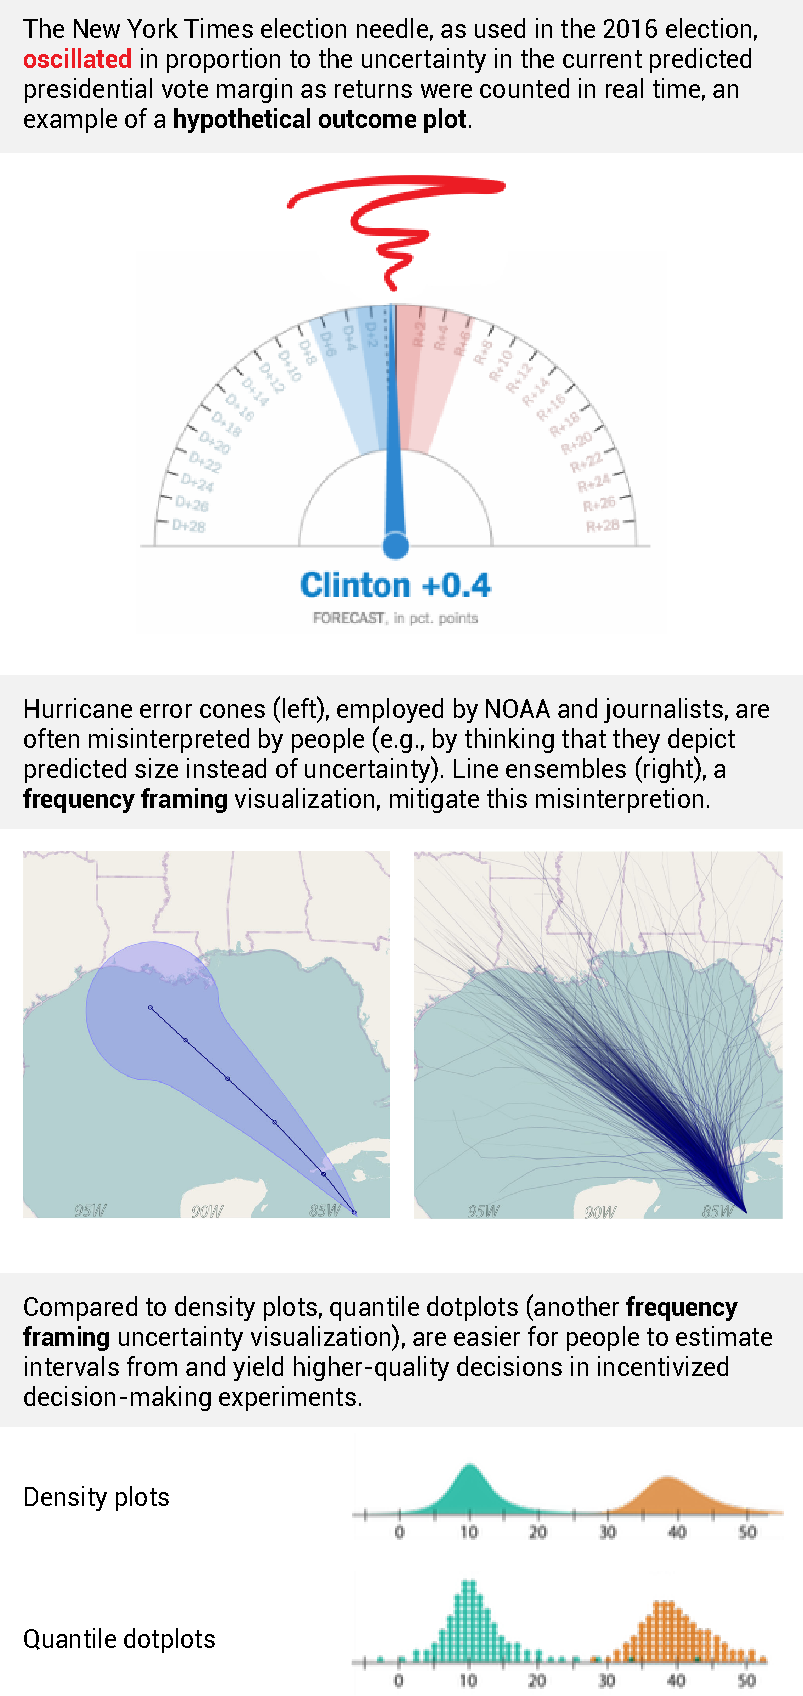
\includegraphics[width=0.5\columnwidth]{img/examples}
  \caption{
    Examples of several uncertainty visualizations one might like to support in a probabilistic grammer of graphics.
  }
  \label{fig:examples}
\end{wrapfigure}

}

\newcommand\figprobgg{

\begin{center}
  \noindent 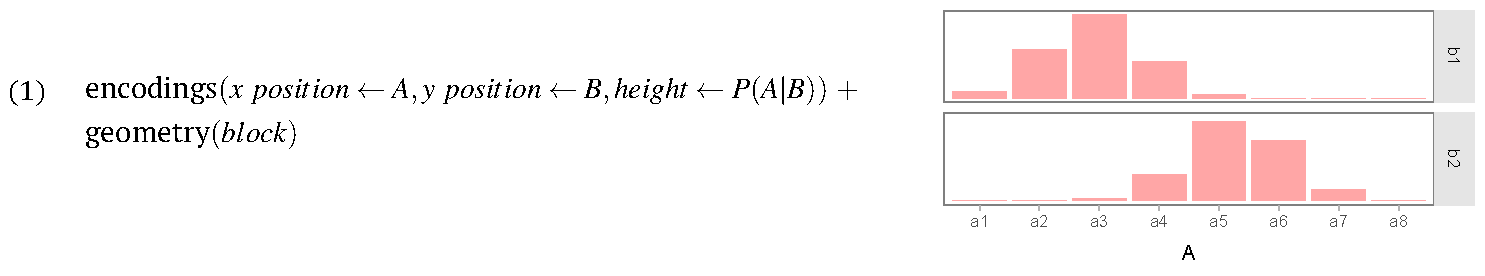
\includegraphics[width=\columnwidth]{img/probgg/prob_gg-1}
  \label{fig:probgg}
\end{center}

\begin{center}
  \noindent 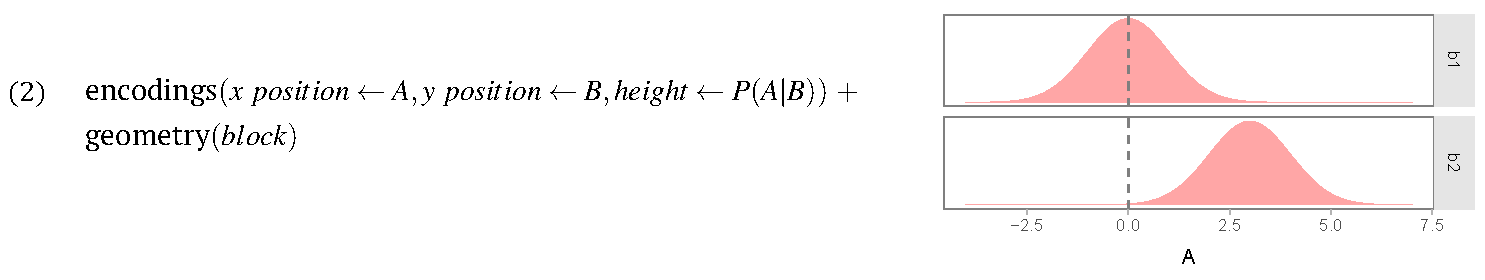
\includegraphics[width=\columnwidth]{img/probgg/prob_gg-2}
  \label{fig:probgg}
\end{center}

\begin{center}
  \noindent 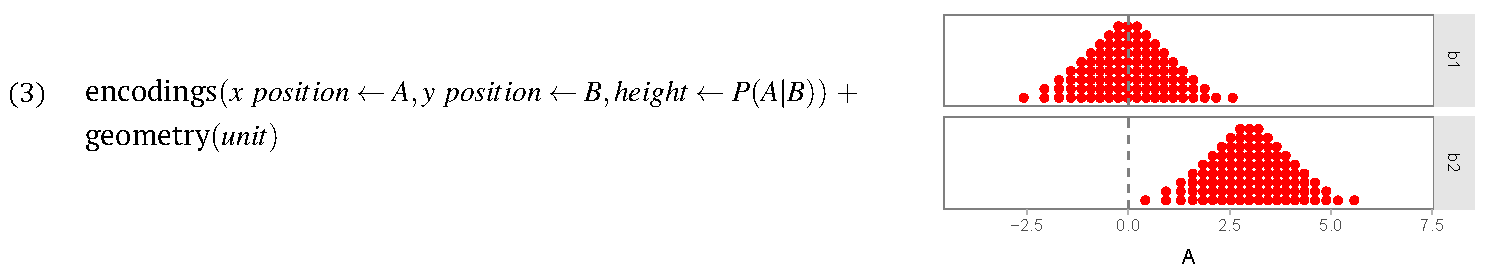
\includegraphics[width=\columnwidth]{img/probgg/prob_gg-3}
  \label{fig:probgg}
\end{center}

}

\newcommand\figboys{

\begin{figure}
  \centering
  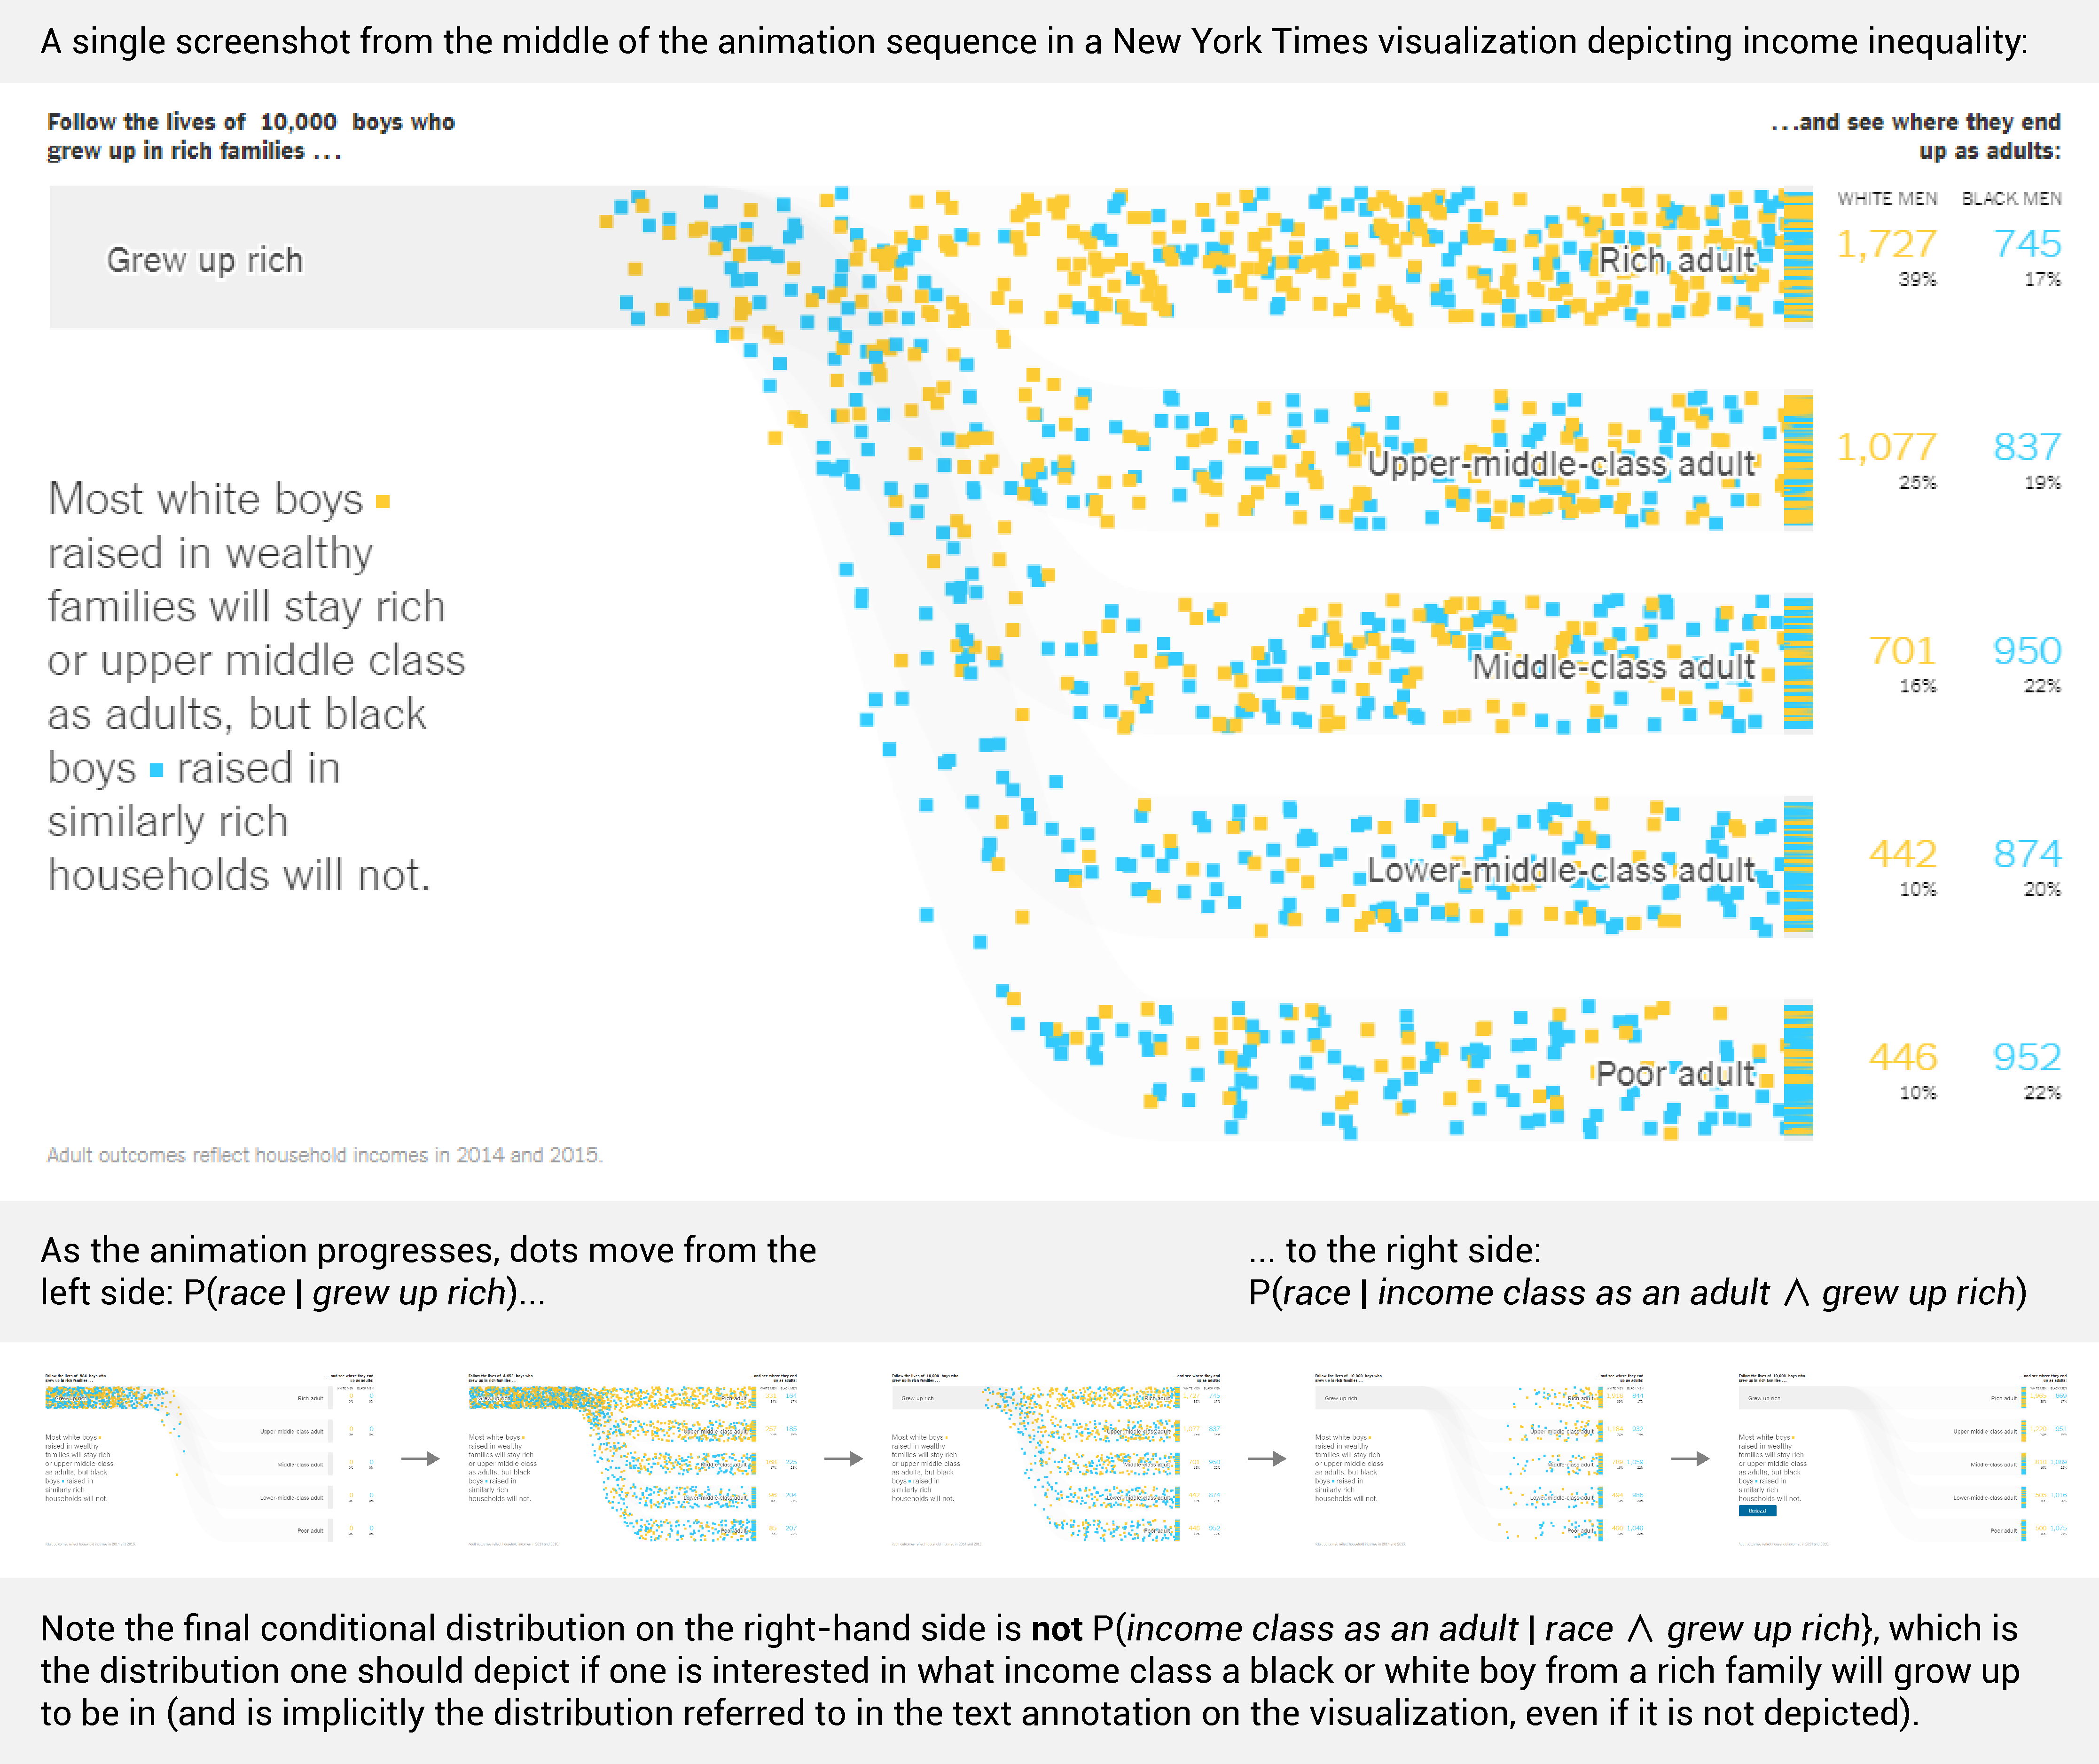
\includegraphics[width=\columnwidth]{img/black-boys/black-boys}
  \caption{
    An example of a professionally-produced probabilistic visualization \cite{badger2018extensive} 
    (\url{https://nyti.ms/2GGpFZw})
    I would both like to be able to support \textbf{and} improve. This visualization falls victim to the \emph{fallacy of the transposed conditional}: by normalizing bar heights on the right-hand 
    side, it depicts $P(race|income~class \wedge grew~up~rich)$ only, so one cannot see 
    $P(income~class | race \wedge grew~up~rich)$: imagine if very few boys of either race who grew up rich ended up in a lower class, then $P(income~class \neq rich | race = black \wedge grew~up~rich)$ would be low even if $P(race = black | income~class \neq rich \wedge grew~up~rich)$ is high. It is worth noting that by reading the numbers in the table to the right it is possible to verify that this is not the case for this particular visualization, but this is difficult to verify from the visualization alone. A probabilistic grammar of graphics would have users explicitly specify the desired distributions, avoiding this error, and would create a similar animation sequence automatically, where this example was custom built in JavaScript.
  }
  \label{fig:boys}
\end{figure}

}





\newcommand\figsystem{

\begin{figure}
  \centering
  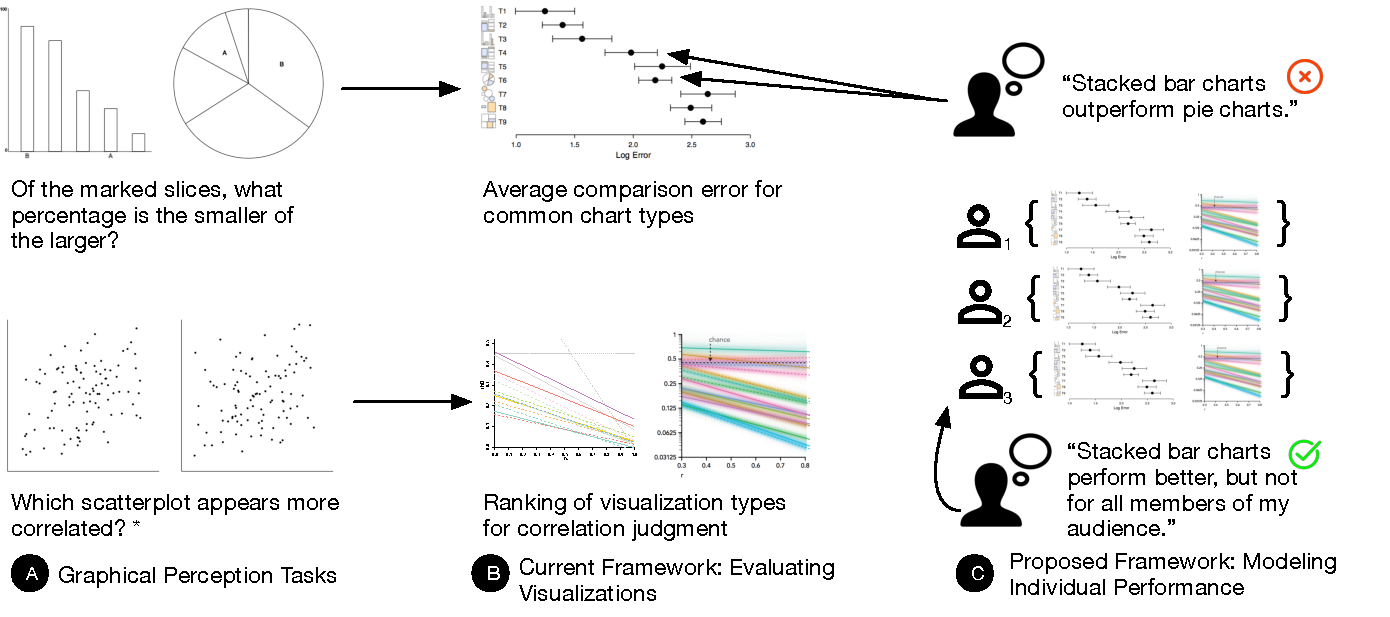
\includegraphics[width=\columnwidth]{old-img/exp-model}
  \caption{
    We propose a new model for graphical perception experiments. A and B illustrate the current model of experiments, where competing visualization designs are evaluated and performance reported for the \emph{average} participant, which by definition leads to overly stringent and possibly incorrect design recommendations in the visualiztion community. C illustrates our proposed framework, in which we \emph{transform} the focus of visualization experiments from evaluating charts to evaluating people, using scalable experiment designs and robust statistical measures. We evaluate our framework using multiple established experiments across diverse participant pools. We evaluate our results through a focused interview study with visualization practitioners. This new model moves to improve and tighten the feedback loop in visualization research, transforming experiments from artifacts to design assets for effective communication through data visualization.
    (*~Can you spot which is most correlated? Our experiments target differences in abilities like this. See the last figure for the answer.)
  }
  \label{fig:system}
\end{figure}

}

\newcommand\figraone{

  \begin{wrapfigure}{r}{0.5\columnwidth}
  \centering
  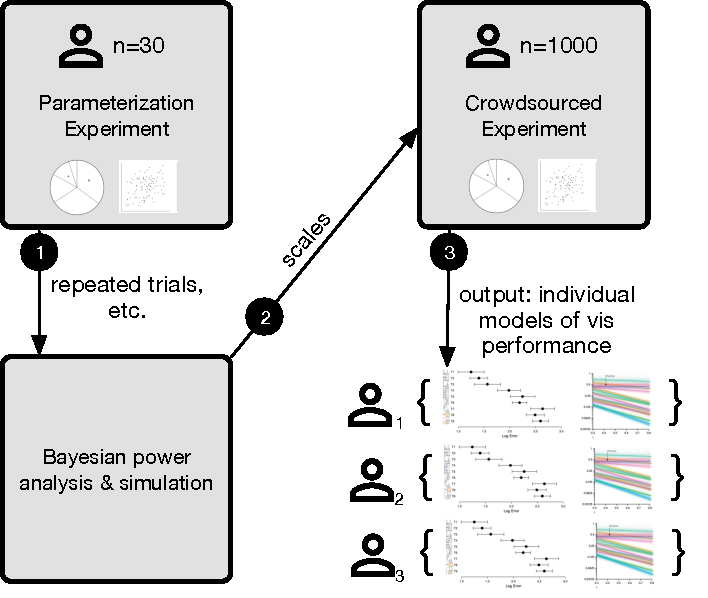
\includegraphics[width=0.48\columnwidth]{old-img/ra1}
  \caption{
    Experiment model for RA1. To evaluate individual differences in visualization performance, we replicate and augment two previously established visualization experiments. We add factors including homogeneous datasets and repeated measures to support between participant comparison and modeling (1). We employ a simulation study (2) to determine parameters for a large crowdsourced experiment with a more diverse population (3).
  }
  \label{fig:ra1}
\end{wrapfigure}

}

\newcommand\figratwo{

  \begin{wrapfigure}{r}{0.5\columnwidth}
  \centering
  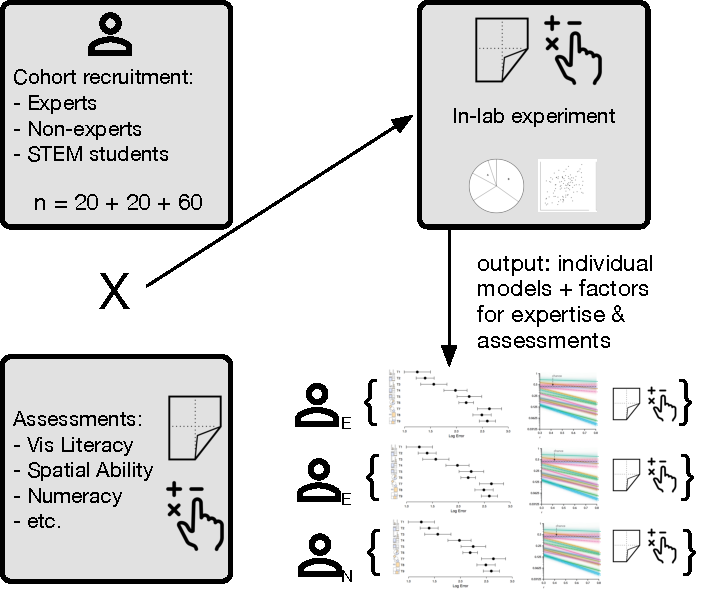
\includegraphics[width=0.48\columnwidth]{old-img/ra2}
  \caption{
    Experiment model for RA2. We explicitly target hypothesized correlates of visualization performance, including expertise, cognitive abilities, and related assessments. We adopt the validated experiment from RA1 as a baseline for an in-lab study, integrate assessments, and extend our robust modeling methodology to evaluate demographics and assessments.
  }
  \label{fig:ra2}
\end{wrapfigure}

}

\newcommand\figrathree{

  \begin{wrapfigure}{r}{0.5\columnwidth}
  \centering
  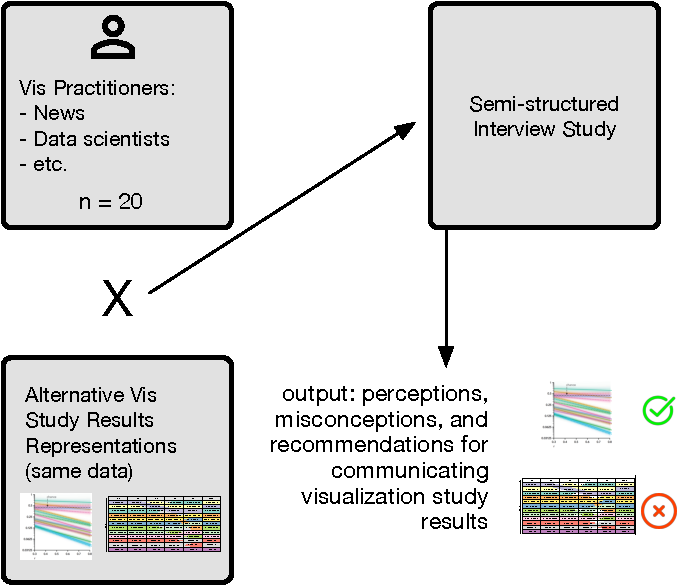
\includegraphics[width=0.48\columnwidth]{old-img/ra3}
  \caption{
    Experiment model for RA3. We challenge longstanding practices in communicating visualization study results. We design alternative representations of study results based on prior work including statistical misconceptions and uncertainty visualization. In an interview study with practitioners, we evaluate how representations shape inferred design guidance that permeates the visualization community.\\
    (*~In Figure \ref{fig:system}, the left scatterplot is most correlated, $r=0.35~v.~0.3$.)
  }
  \label{fig:ra3}
\end{wrapfigure}

}
